\frame{\frametitle{Model Image}
\begin{figure}
	\centering
   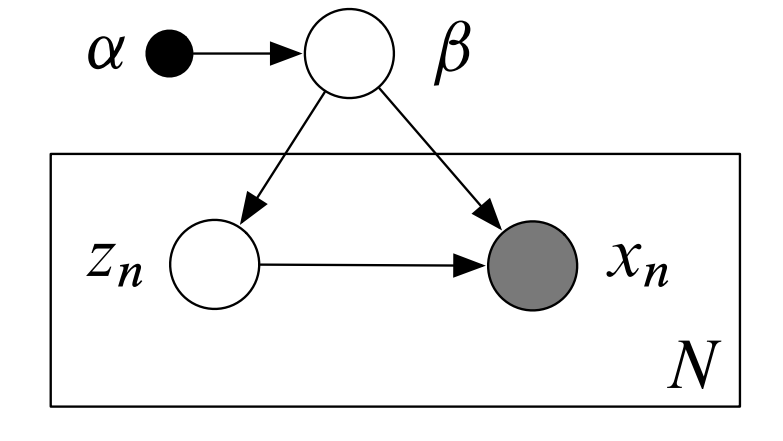
\includegraphics[scale=.25]{figs/fig2-model}
\end{figure}

\begin{table}
\begin{tabular}{cccc}
\textbf{Variable (Hoffman)} & \textbf{Known?} & \textbf{Variable (Jason)} & \textbf{Examples}\\
$x_n$ & observed & input & examples\\
$z_n$ & latent & & ??\\
$\beta$ & latent & nuissance & ??\\
$\alpha$ & either & d& d\\
\end{tabular}
\end{table}
%give gloss of variables: relate them to the input/output/nuissance ones Jason defines
}